\documentclass[12pt]{article}
\usepackage[utf8]{inputenc}
\usepackage[portuguese]{babel}
\usepackage{amsmath,bm,bbm} 
\usepackage{graphicx}
\usepackage{etoolbox}
\usepackage{url}     
\usepackage{changepage}
\usepackage{titlesec}
\usepackage[parfill]{parskip}
\usepackage[margin=1in]{geometry}
\usepackage{times}
\usepackage{float}
\usepackage{cite}
\usepackage[numbers,super]{natbib}
\usepackage{lipsum} 
\titleformat*{\section}{\normalsize\bfseries}
\font\myfont=cmr10 at 10pt

%----------------------------------------------------------------------------------------
%  TITLE SECTION
%----------------------------------------------------------------------------------------
\title{\large \textbf{Ferramentas para Análise de Séries Temporais com Distâncias Estocásticas e Diferenças de Entropias}}
\author{\myfont Eduarda T.\ C.\ Chagas$^{1}$, Alejandro C.\ Frery$^{2}$\\
    \myfont $^{1}$Estudante de IC de Ciência da Computação, Ufal\\
    \myfont $^{2}$Pesquisador do Laboratório de Computação Científica e Análise Numérica, Ufal}
\date{}

\makeatletter 
\patchcmd{\@maketitle}{\begin{center}}{\begin{adjustwidth}{0.5in}{0.5in}\begin{center}}{}{}
\patchcmd{\@maketitle}{\end{center}}{\end{center}\end{adjustwidth}}{}{}
\makeatother

%----------------------------------------------------------------------------------------

\begin{document}
\raggedright
\maketitle
\thispagestyle{empty}
\pagestyle{empty}

%----------------------------------------------------------------------------------------
%  PAPER CONTENTS
%----------------------------------------------------------------------------------------
%Descreva os pontos principais do trabalho incluindo o(s) objetivo(s) de forma clara. Limite de 1000 caracteres contando espaços. 
\textbf{Resumo}

Este trabalho relata o processo de desenvolvimento de uma plataforma de análise de descritores causais de séries temporais oriundos da Teoria da Informação.
A plataforma facilita a análise dessas séries nos mais variados ramos da ciência, como por exemplo, a discriminação entre fenômenos estocásticos e caóticos~\cite{DistinguishingNoiseFromChaos}, a identificação de padrões de comportamento em redes veiculares~\cite{CharacterizationVehicleBehaviorInformationTheory}, a classificação e verificação de assinaturas \textit{online}~\cite{ClassificationVerificationOnlineHandwrittenSignatures}, a análise da robustez de redes~\cite{InformationTheoryPerspectiveNetworkRobustness}, e a classificação de padrões de consumo de energia elétrica~\cite{CharacterizationElectricLoadInformationTheoryQuantifiers}.
O sistema foi implementado na linguagem de programação \texttt R que, além de fornecer ferramentas gráficas, possui a precisão numérica requerida. 
Ambas características são de extrema importância ao longo deste trabalho.
Após comentar brevemente a respeito de conceitos da Teoria da Informação necessários no processo de análise e modelagem de uma série temporal, expomos os resultados alcançados no decorrer do projeto e sugestões para futuros trabalhos.

%------------------------------------------------
%Informe a autorização legal para execução da pesquisa: as referências do cumprimento das exigências legais, com expedição de autorizações junto a Comitês de Ética ou Órgãos Ambientais, número de autorizações ou protocolos expedidos pelo CEP/CONEP, CEUA, IBAMA, ICMBio, CGEN, IPHAN etc.).
\textbf{Autorização legal:} Não se aplica.

%------------------------------------------------
%Informar 3, separadas por ponto e vírgula. Limite 60 caracteres cada. As palavras-chaves do trabalho não podem estar contidas no título do trabalho.
\textbf{Palavras-chave:} Teoria da Informação, plataforma \texttt R, Estatística Computacional.


%------------------------------------------------

\textbf{Apoio financeiro:} CNPq (Conselho Nacional de Desenvolvimento Científico e Tecnológico).


%------------------------------------------------
%Apresentar visão geral sobre o tema, com as justificativas. Incluir o(s) objetivo(s) de forma clara no último parágrafo. Limite 2500 caracteres com espaços. 
\textbf{Introdução}

Séries temporais são conjunto de dados obtidos a partir de um processo observacional ao longo de um determinado período de tempo, não necessariamente dividido em espaços iguais, sendo caracterizadas pela dependência serial existente entre as observações.
 
O estudo de séries temporais é tipicamente dividido em duas vertentes \cite{BrockwellDavis91}: a análise nos domínio do tempo e da frequência, sendo que ambas abordagens empregam os dados que resultam diretamente das observações coletadas, que por sua vez estão sujeitos a efeitos danosos de diversos tipos de contaminação. 
Uma solução alternativa, presente na literatura, para evitar os efeitos dessa contaminação, consiste no uso de métodos não paramétricos.

Há diversas ferramentas que auxiliam na análise clássica de séries temporais para a plataforma \texttt  R (ver \url{https://cran.rproject.org/web/views/TimeSeries.html}). 
Além destas opções, o usuário também pode contar com ferramentas de visualização de séries temporais. No entanto, são limitadas as opções que trabalham exclusivamente com técnicas não paramétricas. 
    
O projeto aqui relatado tomou como ponto de partida a identificação das necessidades dos pesquisadores: uma ferramenta gráfica amigável e funcionalidades rápidas, eficientes e numericamente confiáveis.
Outro requisito foi o da portabilidade para diversos sistemas operacionais e arquiteturas de hardware, e o uso de ferramentas FLOSS (\textit{Free/Libre Open Source Software}).
 
Apresentamos, assim, o desenvolvimento de uma ferramenta portável, rápida e de boa qualidade numérica que possibilita análises interativas e exploratórias de séries temporais através de técnicas provenientes da Teoria da Informação.
Com ela, o usuário dispõe de uma conjunto técnicas de análise presentes na literatura para processar e examinar seus dados de modo eficiente e com um mínimo período de aprendizado.
A ferramenta é extensível.

%------------------------------------------------
%Descreva como o trabalho foi realizado (procedimentos / estratégias; os sujeitos / participantes / documentos; equipamentos / ambientes; etc).Limite 3000 caracteres com espaços
\textbf{Metodologia}

A primeira parte do projeto consistiu da apropriação do referencial teórico.
Seja a série temporal $\bm x = (x_1, x_2, \dots, x_n)$.
Ao invés de analisarmos os valores, transformaremos grupos de $N$ valores (não necessariamente adjacentes) em padrões ordinais, e analisaremos a sua distribuição de frequência.
Por exemplo e sem perda de generalidade, com $N=3$ e para qualquer $i$ viável,
se $x_i<x_{i+1}<x_{i+2}$ assignaremos a esta tripla o padrão $\pi_0$;
caso $x_i>x_{i+1}>x_{i+2}$ o padrão será $\pi_1$ e assim por diante.
Com isso, há $N!$ possíveis padrões.
Esta é conhecida como \textit{simbolização de Bandt \& Pompe}~\cite{PermutationEntropyBandtPompe}.

Forma-se, então, um histograma e, a partir dele, extraem-se quantificadores como, por exemplo, entropia, distância estocástica a uma distribuição de equilíbrio, e complexidade estatística.

Seja, assim, $\bm h=(h_1,\dots,h_{N!})$ o histograma de proporções dos $N!$ padrões observados a partir da série temporal $\bm x$.
Calculamos a entropia de Shannon
\begin{equation}
H(\bm h) = -\sum_{i=1}^{N!} h_i\log h_i,
\label{eq:Entropia}
\end{equation}
com a convenção $-\infty \cdot 0=0$.
A entropia de Shannon é o primeiro elemento a descrever a nossa série temporal.
Ela mede a desordem do sistema que deu origem aos dados $\bm x$.

Calculamos logo a distância de Jensen-Shannoon à distribuição uniforme $\bm u=(1/N!,\dots,1/N!)$
\begin{equation}
D(\bm h,\bm u) = \sum_{i=1}^{N!} \Big(h_i \log\frac{h_i}{u_i} +
u_i \log\frac{u_i}{p_i}
\Big),
\end{equation}
em que $u_i=1/N!$.
Esta é uma medida de quão perto ou longe a dinâmica subjacente está de um processo sem informação nenhuma.

Finalmente, calculamos o terceiro descritor da nossa série temporal: a sua Complexidade Estatística:
\begin{equation}
C(\bm h, \bm u) = H(\bm h) D(\bm h, \bm u).
\end{equation}

Cada série temporal pode então ser descrita por um ponto $(H(\bm h), C(\bm h, \bm u))$.
O conjunto de todos os pares $(H(\bm h), C(\bm h, \bm u))$ para qualquer série temporal descrita por padrões de comprimento $N$ jaz em um subconjunto compacto $\mathbbm R^2$: o plano Entropia-Complexidade.

Embora aqui relatemos apenas o uso da entropia de Shannon e da distância de Jensen-Shannon, o sistema oferece outras entropias~\cite{salicruetal1993} e distâncias estocásticas~\cite{StatisticalInferenceBasedonDivergenceMeasures}.
Com essa contribuição do nosso sistema, as análises podem ser enriquecidas por outros descritores.
 
 Durante o desenvolvimento deste trabalho foram estudadas diversas técnicas de análise de séries temporais, com foco nas ferramentas disponíveis na plataforma \texttt R.
 Após o período inicial de aprendizagem, seguido do levantamento dos requisitos do software, foi iniciada a implementação em \texttt R, usando o software livre de desenvolvimento integrado RStudio Desktop.

%------------------------------------------------
%Limite de 2000 caracteres contando espaços. Se necessário, é permitido ultrapassar este limite, desde que o tamanho total do documento não ultrapasse 4 páginas
\textbf{Resultados e Discussão}

Seguindo o modelo de engenharia de software em espiral, o sistema foi projetado e desenvolvido de forma modular, composto pelas seguintes unidades:

\begin{itemize}
\item Módulo de simbolização;
\item Módulo de análise;
\item Modulo de visualização e interação (em fase de desenvolvimento);
\end{itemize} 

Esses módulos foram e estão sendo desenvolvidos seguindo um cronograma. Depois passaram pelas seguintes etapas:

\begin{itemize}
\item Integração dos módulos em um sistema;
\item Teste e validação do sistema (em fase de desenvolvimento);
\item Geração da interface gráfica (em fase de desenvolvimento).
\end{itemize}

Permite-se a leitura de dados em vários formatos (TXT, CSV ou XLSX), e o usuário a seguir poderá escolher:

\begin{itemize}

	\item Gerar o gráfico da série;
	\item Calcular seus diversos valores de Entropia;
	\item Calcular seus diversos valores de Distâncias estocásticas;
	\item Calcular complexidades estatísticas;
    \item Identificar padrões no gráfico da série temporal;
    \item Gerar planos de Entropias;
    \item Gerar planos de Distâncias estocásticas;
	\item Gerar o histograma de padrões;
	\item Identificar o ponto característico da série no plano Entropia-Complexidade (ver Figura 1).

\end{itemize}

Um elemento original do sistema é a vinculação entre o histograma de padrões e a série temporal. Escolhendo um ou mais elementos do histograma, os valores correspondentes na série temporal aparecem realçados. Esta funcionalidade permite a análise visual da distribuição temporal dos padrões, possibilitando futuramente a realização de outros testes.
 
 O teste e a validação do sistema são tarefas contínuas, bem como o desenvolvimento de novas funcionalidades. 
 
%\begin{figure}[H]
%	\centering
%	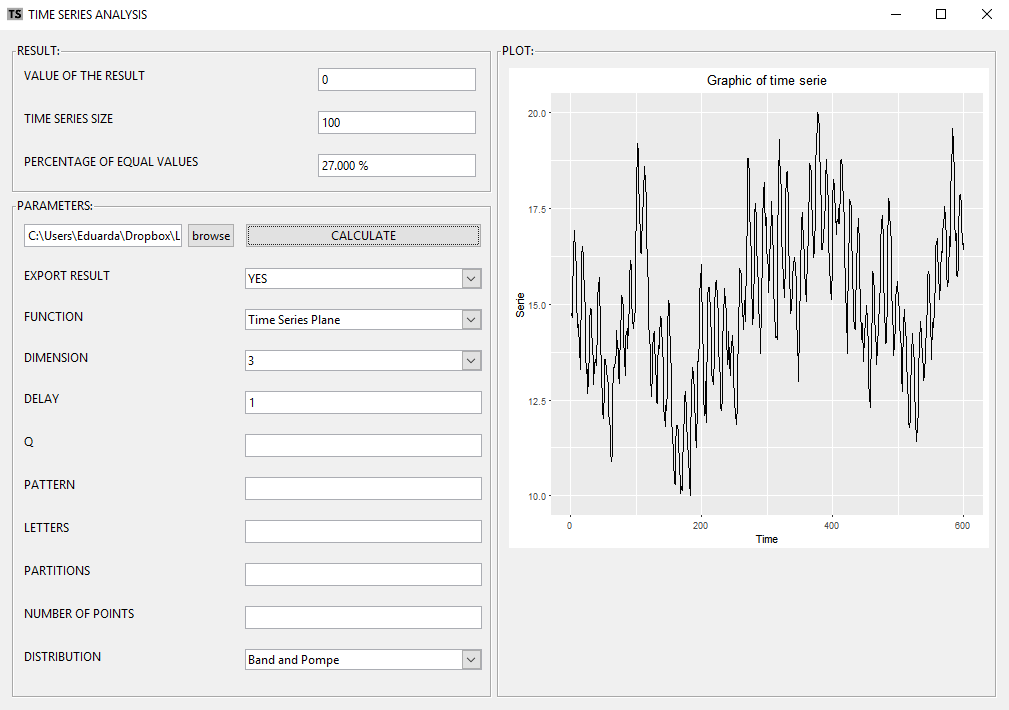
\includegraphics[width=0.85\columnwidth]{TMS}   
%   \caption{Imagem atual do software em processo de desenvolvimento.}
%\end{figure}


%------------------------------------------------
%Limite de 1000 caracteres contando espaços. Se necessário, é permitido ultrapassar este limite, desde que o tamanho total do documento não ultrapasse 4 páginas.
\textbf{Conclusões}

	Através do desenvolvimento de tal plataforma por meio da linguagem \texttt R, fornecemos a base de geração de inúmeros outros modelos que tenham como objetivo a implementação de sistemas confiáveis que tornem mensuráveis as variadas propriedades presentes na teoria da informação, facilitando não apenas o estudo de séries temporais, como também todo o ramo atuante de análise de dados estatísticos.

%-------------------------------------------------------------------
%  REFERENCE LIST
%Descreva as principais referências bibliográficas.
%-------------------------------------------------------------------
%\vspace{4\baselineskip}\vspace{-\parskip} 
%\footnotesize
\bibliographystyle{unsrt} 
\bibliography{ref}

%----------------------------------------------------------------------------------------

\end{document}
